\section{Results}
\label{sec:results}
The results follow the endpoints: first the decomposition of the damage per ratio, then the acceleration, the classes on which each factor's damage lands, the effect of logit adjustment, and finally the selected regularization and temperatures. The balanced arm reaches 72.06 percent balanced accuracy (70.68 to 73.31), as in the prevalence curve.

\subsection{Decomposition of the damage}
\label{sec:decomposition-results}
The prior alone accounts for most of the damage at moderate ratios, the thin support alone for none of it, and at large ratios the two factors together cost far more than their sum (Table~\ref{tab:decomposition}, Figure~\ref{fig:component}). Up to $\rho=20$ the prior-only damage follows the full damage closely: 0.49 against 0.57 points at $\rho=10$, 0.73 against 1.01 points at $\rho=20$. The support-only arm stays within 0.1 points of the balanced arm over the same range, and its intervals contain zero from $\rho=2$ to 20. A balanced objective on the long-tailed rows therefore loses nothing as long as the tail class keeps at least five patches per patient.

\begin{table}[htbp]
\centering
\small
\setlength{\tabcolsep}{4pt}
\renewcommand{\arraystretch}{1.15}
\begin{tabular}{@{}lllllrr@{}}
\toprule
$\rho$ & $\Delta_\text{r}$ (both) & $\Delta_\text{P}$ (prior) & $\Delta_\text{S}$ (support) & Interaction $I$ & Share P & Share S \\
\midrule
2 & 0.11 [0.01, 0.21] & 0.10 [$-$0.00, 0.21] & 0.01 [$-$0.03, 0.04] & 0.01 [$-$0.06, 0.08] & --- & --- \\
5 & 0.37 [0.14, 0.60] & 0.30 [0.09, 0.51] & 0.01 [$-$0.04, 0.06] & 0.06 [0.01, 0.15] & --- & --- \\
10 & 0.57 [0.30, 0.84] & 0.49 [0.25, 0.73] & $-$0.06 [$-$0.13, 0.02] & 0.14 [0.07, 0.21] & --- & --- \\
20 & 1.01 [0.67, 1.36] & 0.73 [0.45, 1.02] & $-$0.07 [$-$0.16, 0.02] & 0.34 [0.24, 0.45] & 0.73 & $-$0.07 \\
50 & 1.85 [1.47, 2.24] & 0.97 [0.65, 1.28] & 0.17 [0.04, 0.31] & 0.71 [0.57, 0.85] & 0.52 & 0.09 \\
100 & 2.91 [2.48, 3.34] & 1.20 [0.87, 1.53] & 0.53 [0.36, 0.70] & \textbf{1.18} [1.00, 1.37] & 0.41 & 0.18 \\
\bottomrule
\end{tabular}
\caption{The skewed prior carries most of the damage up to $\rho=20$; beyond it the interaction of prior and thin support grows fastest. Damages are balanced-accuracy losses against the balanced arm in percentage points, with paired 95\% bootstrap intervals; the interaction is $\Delta_\text{r}-\Delta_\text{P}-\Delta_\text{S}$. Shares are single-factor damages as fractions of $\Delta_\text{r}$ and are omitted where $\Delta_\text{r}<1$ point. Their intervals at $\rho=100$ are 0.34 to 0.48 for P and 0.13 to 0.23 for S.}
\label{tab:decomposition}
\end{table}

\noindent Beyond $\rho=20$ the picture changes. Support alone starts to cost accuracy, 0.17 points at $\rho=50$ and 0.53 points at $\rho=100$, when the tail class keeps between one and three patches per patient. The prior-only damage keeps growing slowly and reaches 1.20 points at $\rho=100$. The interaction is resolved from $\rho=5$ on and roughly doubles with each step of the grid, from 0.14 points at $\rho=10$ to 1.18 points at $\rho=100$, where it is as large as the prior-only damage. At the primary ratio the prior accounts for 41 percent of the full damage, support for 18 percent, and the interaction for the remaining 41 percent. The three splits agree: the interaction at $\rho=100$ is 1.29, 1.07, and 1.20 points.

\begin{figure}[htbp]
\centering
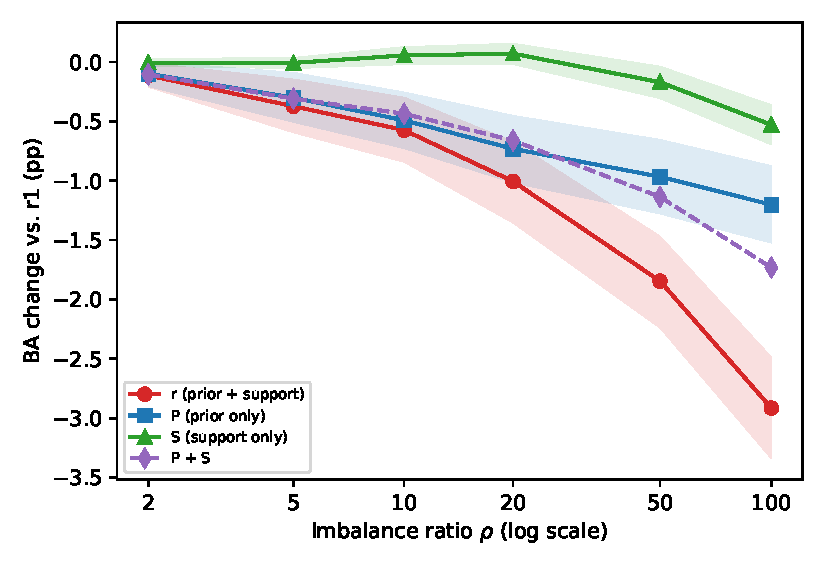
\includegraphics[width=0.6\textwidth]{component.pdf}
\caption{The full damage exceeds the sum of its single-factor parts at every ratio beyond $\rho=10$. Change in patient-macro balanced accuracy relative to the balanced arm for the ratio arm r (prior and support), the prior-only arm P, and the support-only arm S, each with a shaded paired 95\% bootstrap band; the dashed line is the sum of the P and S changes. All series are plotted at the realized ratio of r$\rho$.}
\label{fig:component}
\end{figure}

\subsection{Acceleration}
\label{sec:acceleration-results}
The three families accelerate differently (Table~\ref{tab:slopes}). The full damage grows by 0.18 points per doubling of $\rho$ up to $\rho=10$ and by 0.70 points beyond, an acceleration of 0.52 points (0.44 to 0.60). The prior-only damage is close to linear in $\log\rho$: 0.17 points per doubling below $\rho=10$ and 0.21 above, a difference of 0.04 points whose interval contains zero. The support-only damage is flat below $\rho=10$ and grows by 0.18 points per doubling above it, a resolved acceleration of 0.20 points (0.16 to 0.24). The single factors together account for 0.24 of the 0.52 points of acceleration; the rest comes from the growing interaction.

\begin{table}[htbp]
\centering
\renewcommand{\arraystretch}{1.15}
\begin{tabular}{@{}llll@{}}
\toprule
Family & Slope, $\rho\leq10$ & Slope, $\rho\geq10$ & Acceleration \\
\midrule
r (both) & 0.18 [0.09, 0.26] & 0.70 [0.63, 0.76] & \textbf{0.52} [0.44, 0.60] \\
P (prior) & 0.17 [0.08, 0.25] & 0.21 [0.17, 0.25] & 0.04 [$-$0.02, 0.11] \\
S (support) & $-$0.02 [$-$0.05, 0.00] & 0.18 [0.13, 0.22] & \textbf{0.20} [0.16, 0.24] \\
\bottomrule
\end{tabular}
\caption{The prior-only damage grows at a constant rate per doubling, while the support-only damage appears only beyond $\rho=10$. Least-squares slopes of the damage on $\log_2\rho$ in points per doubling, with paired 95\% bootstrap intervals; acceleration is the high-segment slope minus the low-segment slope, in bold where resolved above zero. The low segment of r includes the balanced arm at $\rho=1$; those of P and S start at $\rho=2$.}
\label{tab:slopes}
\end{table}

\subsection{Where the damage lands}
\label{sec:rank-results}
Both factors move recall from the tail third of the classes to the head third, but they do so in different proportions, and neither reaches the redistribution of the ratio arm (Table~\ref{tab:thirds}). At $\rho=100$ the prior-only arm lowers tail recall by 5.9 points and raises head recall by 3.2 points, and the support-only arm lowers the tail by 3.7 and raises the head by 2.0, although its objective is balanced. The ratio arm lowers the tail by 11.8 points, 2.2 points more than the two single-factor losses together, and it also lowers the body by 2.3 points, where the single-factor arms lose 0.8 points or nothing. The interaction thus falls mainly on the tail and body, not on the head, whose gains are close to additive. Below $\rho=20$ the support-only arm leaves all three thirds within one point of the balanced arm, whereas the prior-only arm already shifts 4.1 points of tail recall at $\rho=10$.

\begin{table}[htbp]
\centering
\small
\renewcommand{\arraystretch}{1.15}
\begin{tabular}{@{}lrrrrrrrrrr@{}}
\toprule
 & & \multicolumn{3}{c}{$\rho=10$} & \multicolumn{3}{c}{$\rho=20$} & \multicolumn{3}{c}{$\rho=100$} \\
\cmidrule(lr){3-5}\cmidrule(lr){6-8}\cmidrule(lr){9-11}
Third & r1 & r & P & S & r & P & S & r & P & S \\
\midrule
Head & 72.06 & 76.12 & 74.98 & 72.75 & 76.58 & 75.00 & 73.13 & 77.48 & 75.21 & 74.10 \\
Body & 72.19 & 71.48 & 71.87 & 72.12 & 71.00 & 71.67 & 72.05 & 69.87 & 71.36 & 72.28 \\
Tail & 71.92 & 66.85 & 67.84 & 71.47 & 65.57 & 67.31 & 71.20 & 60.08 & 65.99 & 68.21 \\
\bottomrule
\end{tabular}
\caption{The combination of prior and thin support costs the tail more than the two factors separately. Mean patient-macro recall in percent of the ten head, body, and tail classes of each draw, by their assigned rank, averaged over 30 fits. The r columns are taken from the prevalence curve.}
\label{tab:thirds}
\end{table}

\subsection{Logit adjustment}
\label{sec:adjustment-results}
Post-hoc logit adjustment repairs part of the ratio arm's damage but none of the prior-only arm's (Table~\ref{tab:adjustment}). Applied to r100, it raises balanced accuracy from 69.14 to 70.61 percent and removes about half of the 2.91-point damage. It still falls 0.92 points (0.59 to 1.24) short of the support-only arm, which trains on the same rows with a balanced objective, and it falls short of it at every ratio from $\rho=5$ on. Applied to P$\rho$, the same correction lowers balanced accuracy, by 0.49 points at $\rho=100$. The intercept share of the prior damage is therefore negative: at $\rho=50$ and $\rho=100$ the adjustment adds about 40 percent to the prior-only damage (41 percent at $\rho=100$, 13 to 87) instead of removing part of it, and at $\rho\leq20$ its effect is not resolved. Subtracting the full log prior thus overcorrects the prior-only arm. This indicates that the weighted fit has not shifted its class intercepts by the full log prior; its damage lies in how the class weights change the fitted scores, not in a uniform intercept offset.

\begin{table}[htbp]
\centering
\renewcommand{\arraystretch}{1.15}
\begin{tabular}{@{}lrrrrrl@{}}
\toprule
$\rho$ & r & Lr & P & LP & S & Lr $-$ S \\
\midrule
10 & 71.48 & 71.82 & 71.57 & 71.56 & 72.11 & $-$0.30 [$-$0.50, $-$0.09] \\
20 & 71.05 & 71.56 & 71.33 & 71.22 & 72.13 & $-$0.56 [$-$0.82, $-$0.30] \\
50 & 70.21 & 71.25 & 71.09 & 70.70 & 71.89 & $-$0.64 [$-$0.91, $-$0.36] \\
100 & 69.14 & 70.61 & 70.85 & 70.36 & 71.53 & $-$0.92 [$-$1.24, $-$0.59] \\
\bottomrule
\end{tabular}
\caption{Logit adjustment helps the ratio arm but stays below training-time rebalancing, and it hurts the prior-only arm. Test patient-macro balanced accuracy in percent; the balanced arm reaches 72.06. Lr and LP subtract the log training prior from the logits of r and P; the last column is the paired difference between post-hoc and training-time correction of the same rows, with its 95\% bootstrap interval.}
\label{tab:adjustment}
\end{table}

\subsection{Regularization and temperature}
\label{sec:selection-results}
The prevalence curve found that stronger imbalance selects weaker regularization and needs a larger temperature, and it could not say whether the prior or the support causes this \citep{queisler2026prevalenceTcga}. The prior does. The support-only arms select $\lambda=0.1$ in 27 or 28 of 30 fits and $\lambda=0.01$ in the rest at every ratio, like the balanced arm, and their mean temperature stays at 0.85 from $\rho=2$ to 100, against 0.84 for r1. The prior-only arms move toward weaker regularization as $\rho$ grows: $\lambda=0.1$ in 20 of 30 fits at $\rho=2$, $\lambda=0.01$ in 27 of 30 at $\rho=10$, and $\lambda\leq10^{-3}$ in all 30 at $\rho=100$, the same choice as r100. Their mean temperature rises from 0.94 at $\rho=2$ to 1.71 at $\rho=100$, below the 2.35 of r100. Every selection lies inside the grid.

\section{Discussion}
\label{sec:discussion}
Of the readings fixed in Section~\ref{sec:evaluation}, the results select the interaction reading. At $\rho=100$ the prior-only damage exceeds one point but carries only 41 percent of the full damage, the support-only damage stays below one point, and the interaction is resolved at 1.18 points. The same reading holds at $\rho=20$, where the interaction of 0.34 points is resolved and the prior-only damage of 0.73 points falls short of the one-point condition. The acceleration is attributed to support, the only single factor with a resolved slope difference, but the interaction contributes more than half of it.

The two factors thus play different roles along the curve. At moderate ratios, the prevalence damage on TCGA-UT is a prior effect: a balanced objective on the long-tailed rows loses nothing up to $\rho=20$, so five patches per patient are enough to estimate a tail class once its share of the loss is restored. The prior alone produces a steady loss of about 0.2 points per doubling of $\rho$, together with the shift toward weaker regularization and higher temperature. At large ratios the two factors compound. A skewed prior costs 1.20 points when every class keeps 640 patches, but 1.20 plus 1.18 points when the tail is also thin. A plausible mechanism is that a tail class estimated from one or two patches per patient has noisy and weak scores, so the head-ward push of the prior moves more of its test patches across the boundary than it does for a well-estimated class. The tail and body losses of Table~\ref{tab:thirds}, which exceed the single-factor sum while the head gains do not, fit this account. The study does not test the mechanism directly.

For mitigation, the decomposition points to training-time rebalancing. On the rows of r$\rho$, restoring a balanced objective by class weights removes the prior damage and the interaction together and leaves only the support-only damage, 0.53 points at $\rho=100$. Post-hoc logit adjustment of the same classifier recovers only half of the damage and stays 0.92 points below that level, and it does not help a classifier whose prior was imposed by weights. On TCGA-UT, the cheap post-hoc correction is therefore not a substitute for rebalancing during training. The support-only damage that remains is small compared with the patient-count effects of this series \citep{queisler2026centreError}.

The companion BRACS study suggested that its large damage comes from a shifted prior under class overlap, not from thin tail support \citep{queisler2026prevalenceBracs}. On TCGA-UT, the prior alone at full support costs at most 1.20 points, far below the 7.65 points of BRACS at $\rho=100$, and the interaction with thin support is as large as the prior effect itself. The BRACS explanation thus needs its own test, with the same design on BRACS, before the prior can be credited with the BRACS damage.

\section{Limitations}
\label{sec:limitations}
The prior-only arm imposes the long-tailed prior by class weights, not by resampling. Its weighted objective has the same expectation as that of the ratio arm, but it is not the same estimator: the head rows of P number 640 rather than up to 2,843, and weighting and sampling can reach different solutions for a regularized classifier, as the adverse effect of logit adjustment on P indicates. The interaction therefore mixes the effect of thin support under a skewed prior with any difference between weighting and sampling. A design that resamples the head at full tail support would separate them, but at a fixed patient depth of 160 patches it is feasible only up to $\rho\approx5$. Each fitted arm selects its own regularization, so the decomposition includes the effect of the prior on model selection; with $\lambda$ held fixed, the prior-only damage could differ.

The acceleration segments of the P and S families start at $\rho=2$, whereas that of the r family starts at $\rho=1$; the low-segment slopes of P and S are therefore estimated from three points. The shares at $\rho=20$ rest on a full damage that meets the one-point threshold only by its point estimate. All results are conditional on twenty patients per class, frozen Virchow2 features, multinomial logistic regression, TCGA-UT, and three overlapping splits.
